\documentclass{../cheat}
\title{3D Computer Vision}
\author{ma.mehralian}

%======
%\def \TitleText {}
\def \itm{{\tiny$\blacktriangleright$}}
%======

\usepackage{float}
\floatstyle{ruled}
\newfloat{tables}{thp}{lop}
\floatname{tables}{Tables}


\begin{document}


%==========================================================
\begin{multicols}{3}

\section{Single-View Geometry}
\subsection{C2: Representation of a 3D Moving Scene}
	\setlength{\gapspace}{0.35\columnwidth}
	\textbf{3D Euclidean Space}
	\begin{itemize}
		\item \tab{Inner product:} $\langle u,v \rangle=u^T v \in \mathbb{R}^3$
		\item \tab{Cross product:} $\begin{array}{l}
			u\times v=-v\times u \;\; \in \mathbb{R}^3\\
			u \times (\alpha v+ \beta w)=\alpha u \times v+ \beta u+w
			\end{array} $		
		\item \tab{Skew-symmetric:} $u \times v=\widehat{u}v$\\
			\centerline{$\begin{array}{l}
				\widehat{u} v=
				\begin{bmatrix}	0 & -u_3 & u_2 \\	u_3 & 0 & -u_1 \\	-u_2 & u_1 & 0 \end{bmatrix}
				\begin{bmatrix} v_1 \\ v_2 \\ v_3 \end{bmatrix}
				= \begin{bmatrix} u_2 v_3 - u_3 v_2 \\	u_3 v_1 - u_1 v_3 \\	u_1 v_2 - u_2 v_1	\end{bmatrix} \\
				\left[u\right]_\times=\widehat{u}=-\widehat{u}^T$,  $\widehat{u}u=0, x^T \widehat{u} x=0 \\
				\text{when} \quad \Vert{u}\Vert=1 \quad \text{then} \quad \widehat{u}\;{\widehat{u}}^T\;\widehat{u}= \widehat{u}
				\end{array}$}
		\item \tab{Orthogonality:} $\langle u\times v,v \rangle=\langle u\times v,u \rangle=0$
	\end{itemize}
	
	\textbf{Rotational Motion}
	\begin{itemize}
		\item \tab{Rotational motion:}$R_{cw}=R^{-1}_{wc}=R^{T}_{wc}$
		\item Special Orthogonal group:\\
			\centerline{$SO(3)\doteq\{R\in \mathbb{R}^{3\times3}| R^T R=I, det(R)=+1\}$}
		\item \tab{Exponential Map:} 
			$so(3)\doteq \{ \widehat{\omega}\in \mathbb{R}^{3\times3}| \omega \in \mathbb{R}^3 \}$\\
			\centerline{exp: $so(3) \rightarrow SO(3); \quad \widehat{\omega} \mapsto e^{\widehat{\omega}}$}\\
			\centerline{$R=e^{\widehat{\omega}} \quad \widehat{\omega}=log(R)$}\\
			rotating around some fixed axis $\omega$ by a certain angle $\Vert{\omega}\Vert$
		\item \tab{Rodrigues' Formula:}\\
			\centerline{$e^{\widehat{\omega}} = I + \frac{\widehat{\omega}}{\Vert{\omega}\Vert} \sin(\Vert{\omega}\Vert) + \frac{\widehat{\omega}^2}{\Vert{\omega}\Vert^2} (1-\cos(\Vert{\omega}\Vert))$}
	\end{itemize}
	
	\textbf{Rigid-body Motion}
	\begin{itemize}
		\item Special Euclidean group:\\
			\centerline{$SE(3)\doteq\{g=(R,T)|R\in SO(3) , T \in \mathbb{R}^3\}$}
		\item \tab{Motion Composition:}  $\begin{array}{l}
			g(t_3,t_1)=g(t_3,t_2)g(t_2,t_1) \\
			g_{13}=\begin{bmatrix}	R_{12}R_{23} & R_{12}T_{23}+T_{12} \\ 0 & 1 \end{bmatrix}
			\end{array} $
		\item \tab{Motion inverse:} $g(t_2,t_1)^{-1}=g(t_1,t_2)$\\
			\centerline{$g^{-1}=\begin{bmatrix}	R & T \\ 0 & 1 \end{bmatrix}^{-1}=
			\begin{bmatrix}	R^T & -R^T T \\ 0 & 1 \end{bmatrix} \in SE(3)$}
		\item \tab{Exponential Map:} \\
			\centerline{$se(3)\doteq \left\lbrace \widehat{\xi}=
				\begin{bmatrix} \widehat{\omega} & v \\ 0 & 0 \end{bmatrix} \;\middle|\; 
			 	\widehat{\omega} \in so(3), v \in \mathbb{R}^3 \right\rbrace \subset \mathbb{R}^{4\times4} $}\\
		 	\centerline{exp: $\text{se(3)} \rightarrow \text{SE(3)}; \quad \widehat{\xi} \mapsto e^{\widehat{\xi}}$}\\
		 	\centerline{$R=e^{\widehat{\xi}} \quad \widehat{\xi}=log(R)$}
	\end{itemize}


	\textbf{Coordinate and velocity transformation}
	\begin{itemize}
		\item \tab{$X(t)=R(t)X_0+T(t)$} $\dot{X}(t)=\widehat{\omega}X(t)+v(t)$
		\item \tab{Adjoint map} $\widehat{\omega} \mapsto R\widehat{\omega}R^T$
	\end{itemize}
		
	\textbf{Other!!}
	\setlength{\gapspace}{0.3\columnwidth}
	\begin{itemize}
			\item \tab{Euler Angles:} $R=R_z(\alpha) R_y(\beta) R_x(\gamma)$\\
			\centerline{$\begin{bmatrix}
				\cos\alpha & -\sin\alpha & 0 \\
				\sin\alpha & \cos\alpha & 0 \\
				0 & 0 & 1
				\end{bmatrix}\begin{bmatrix}
				\cos\beta & 0 & \sin\beta \\
				0 & 1 & 0\\
				-\sin\beta & 0 & \cos\beta
				\end{bmatrix}\begin{bmatrix}
				1 & 0 & 0\\
				0 & \cos\gamma & -\sin\gamma \\
				0 & \sin\gamma & \cos\gamma		
				\end{bmatrix}$}
		\item \tab{A Unit Quaternion:} $\begin{array}{l c l}
			 \mathbf{q}^{-1} & = & e^{-\tfrac{\theta}{2}{(u_xi + u_yj + u_zk)}}\\
			 & = & \cos \tfrac{\theta}{2}-(u_x\mathbf{i}+u_y\mathbf{j}+u_z\mathbf{k})\sin \tfrac{\theta}{2}
			\end{array}$\\
			A rotation about the unit vector $u$ by an angle $\theta$
		\item Homogeneous coordinates \quad
			$ (x,y) \leftrightarrow  (\lambda x, \lambda y, \lambda ), \quad \forall \lambda \neq 0$
		\item Homogeneous Linear Least Squares problem:\quad $Ax=0$
		\item \tab{Line equation} $ax + by + c = 0$ \\
			\centerline{$\mathbf{x}^\top l = 0,\quad  \textrm{where}\quad l = (a,b,c)^\top$}
		\item \tab{Conic equation} $ax^2+bxy + cy^2 + dxz + eyz + fz^2 = 0$\\
			\centerline{$\mathbf{x}^{\top} C \mathbf{x} = 0, \quad  \textrm{where}\quad C = \begin{bmatrix}
			a & b/2 & d/2 \\  b/2 & c & e/2 \\  d/2 & e/2 & f \end{bmatrix}$}
		\item \tab{Parallel lines} $\begin{array}{l} 
			 l=(a,b,c), l'=(a,b,c') \\
			l\times l'\sim (b,-a,0)
			\end{array}$
		\item \tab{Duality} $p=l_1 \times l_2, \;\; l=p_1 \times p_2$
		\item \tab{Ideal points} $p_\infty=(x_1, x_2, 0)$
		\item \tab{Line at infinity} $l_\infty=(0, 0, 1)$
		\item \tab{Plane at infinity} $\pi_\infty=(0, 0, 0, 1)$
	\end{itemize}	
	
	\textbf{Table 2.1. Rotation and rigid-body motion in 3D space.}\\
	\begin{tabularx}{\columnwidth}{| @{ }p{47pt} | @{ }p{67pt} | X |}
	\hline
	& Rotation SO(3) & Rigid-body motion SE(3) \\ \hline \hline
	Matrix rep &  $R: \left\{ \begin{array}{l}
		R^T R=I\\ det(R)=1	\end{array}\right.$ & $g=\begin{bmatrix}
		R & T\\0 & 1 	\end{bmatrix}$\\ \hline
	Coord (3D) & $X=RX_0$ & $X=RX_0+T$\\ \hline
	Inverse & $R^{-1}=R^T$ & $g^{-1} = \begin{bmatrix}
		R^T & -R^T T\\ 0 & 1 \end{bmatrix}$\\ \hline
	Composition & $R_{ik} = R_{ij} R_{jk}$ & $g_{ik} = g_{ij} g_{jk}$\\ \hline \hline
	
	Exp. rep & $R = exp(\widehat{\omega})$ &  $g = exp(\widehat{\xi})$ \\ \hline
	Velocity & $\dot{X}=\widehat{\omega}X$ & $\dot{X} =\widehat{\omega}X +v$  \\ \hline
	Adjoint map & $\widehat{\omega} \mapsto R \widehat{\omega} R^T$ & $\widehat{\xi} \mapsto g \widehat{\xi} g^{-1}$  \\ \hline
	\end{tabularx}

\subsection{C3: Image Formation}
	\textbf{Camera Model}\\
	
	\centerline{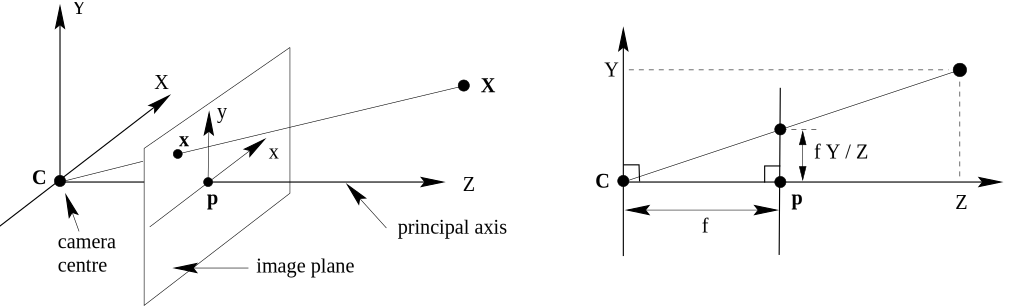
\includegraphics[scale=0.3]{images/camera_fig_6_1}}
	\setlength{\gapspace}{0.45\columnwidth}
	\begin{itemize}
		\item \tab{World $\rightarrow$ Camera:} $X_c=R X_w+T \hspace{12pt}$
		\item \tab{Camera $\rightarrow$ Image Plane:} $x=-f\frac{X}{Z}, y=-f\frac{Y}{Z}$
		\item \tab{Ideal Pinhole Camera} $\pi:\mathbb{R}^3 \mapsto \mathbb{R}^2; \;\; X \mapsto x$
		\item 3D homogeneous coordinates:\\
			\centerline{
			$\lambda\begin{bmatrix}x \\ y \\ 1 \end{bmatrix}=\underbrace{\begin{bmatrix} 
			f & 0 & 0 \\ 0 & f & 0 \\	0 & 0 & 1
			\end{bmatrix}}_{K_f}
			\underbrace{\begin{bmatrix} 
			1 & 0 & 0 & 0 \\ 0 & 1 & 0 & 0\\	0 & 0 & 1 & 0
			\end{bmatrix}}_{\Pi_0}
			\underbrace{\begin{bmatrix} 
			R & &T \\ \\ 0 & &1 \end{bmatrix}\begin{bmatrix} 
			X_0 \\ Y_0 \\ Z_0 \\ 1
			\end{bmatrix}}_{X_c=g_0 X_w}$}
		\item \tab{Image Plane $\rightarrow$ Pixel:} $x'=K_s x$
		\item 3D homogeneous coordinates:\\
			\centerline{$\begin{bmatrix}x' \\ y' \\ 1 \end{bmatrix}=\underbrace{\begin{bmatrix} 
				s_x & s_\theta & o_x  \\ 0 & s_y & o_y \\	0 & 0 & 1
				\end{bmatrix}}_{K_s}
				\underbrace{\begin{bmatrix} 
				x \\ y \\ 1
				\end{bmatrix}}_{\textrm{Metric}}$}\\
			where $s_\theta$= skew factor, $(o_x, o_y)$= principal point in terms of pixel dimensions (center offsets),
				 $f$= focal length, $(s_x, s_y)$= number of pixels per unit distance in image coordinates (scaling factors).
		\item Camera calibration(intrinsic):  $K=K_s K_f$ (5 DOF)
		\item \tab{Camera model:} $X'=K\Pi_0 g X$
		\item \tab{Projection matrix: } $\Pi=K\Pi_0 g=[KR,KT]$\\
			\centerline{$\lambda x'=\Pi X_0$ ($\lambda$: projective dept)}
	\end{itemize}

	
\subsection{C4: Image Primitives and Correspondence}
	\textbf{Small baseline}: feature tracking and optical flow\\
	\centerline{$I_1(x)=I_2(h(x))=I_2(x + \Delta x)$, $\Delta X\doteq \mathtt{u} dt$}
	%\tab{velocity vector:} $\overrightarrow{v}\approx-\frac{I_t}{I_x}$\\
	\tab{image velocity:} $u=-G^{-1}b$ \\
	\centerline{$G=\begin{bmatrix}
		\sum I_x^2 & \sum I_xI_y \\ \sum I_xI_y & \sum I_y^2
		\end{bmatrix}$, $b=\begin{bmatrix}
		\sum I_xI_t \\ \sum I_yI_t
		\end{bmatrix}$}
	\begin{itemize}[nolistsep, leftmargin=1em]
		\item Rank(G) = 0 blank wall problem (flat area)
		\item Rank(G) = 1 aperture problem (line)
		\item Rank(G) = 2 enough texture, good feature candidates
	\end{itemize}
	Similarity measure: Sum of Squared Differences (SSD)\\
	\textbf{Large baseline:} Feature matching\\
	\centerline{$ h(\tilde{x})=\begin{bmatrix}a_1 & a_2 \\ a_3 & a_4\end{bmatrix}
	\tilde{x}+\begin{bmatrix}d_1 \\ d_2\end{bmatrix}$}\\
		Similarity measure: Normalized cross-correlation (NCC)
	
	Point feature selection:	Harris: $C(x)=det(G)+\kappa.trace^2(G)$

\section{Two-View Geometry}

\subsection{C5: Reconstruction from 2 Calibrated Views}
	Epipolar geometry:\\
	\centerline{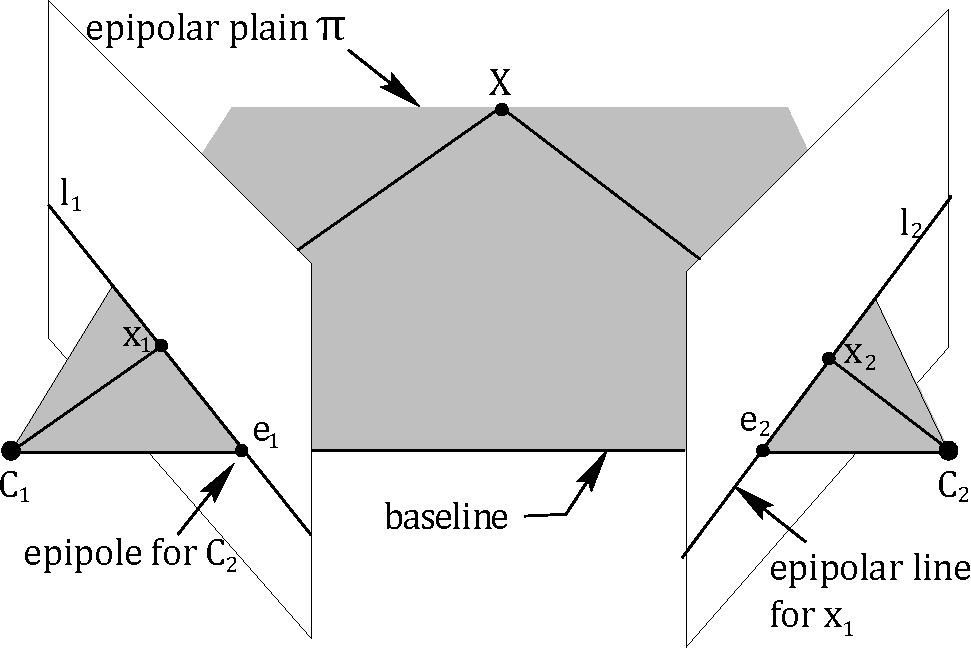
\includegraphics[scale=0.3]{images/epipolar_fig_9_1}}
	
	Pose Recovery from the Essential Matrix:
	\begin{itemize}[nolistsep, leftmargin=1em]
		\item Decompose(SVD): $E=U\Sigma V^T$\\
			where $\Sigma=diag\{\sigma,\sigma,0\}$ and $U,V \in SO(3)$
		\item Calculate two pairs of camera matrices:\\
			\centerline{$(\widehat{T}_1,R_1)=(UR_Z(+\frac{\pi}{2})\Sigma U^T, UR_Z(+\frac{\pi}{2})V^T)$}
			\centerline{$(\widehat{T}_2,R_2)=(UR_Z(-\frac{\pi}{2})\Sigma U^T, UR_Z(-\frac{\pi}{2})V^T)$}
	\end{itemize}
	
	\textbf{The eight-point linear algorithm:}
	\begin{itemize}[nolistsep, leftmargin=1em]
		\item Calculate Kronecker product for each pair: $a=x_1\otimes x_2$\\
			\centerline{$a \doteq [x_1 x_2 ,x_1 y_2 ,x_1 z_2 ,y_1 x_2 ,y_1 y_2 ,y_1 z_2 ,z_1 x_2 ,z_1 y_2 ,z_1 z_2]^T$}
		\item From a set of $n$ point matches, we obtain a set of linear equations of the form\\
			\centerline{$\chi\doteq[a^1, a^2, ..., a^n]^T$}
		\item Solve linear equation:  $\chi E^s=0$ \\
			Where $E^s $ is stacked vector of $E$\\
			\centerline{$E^s\doteq[e_{11}, e_{21}, e_{31}, e_{12}, e_{22}, e_{32}, e_{13}, e_{23}, e_{33}]^T$}
	\end{itemize}
	
	\textbf{Planar scenes and homography}
	$\widehat{e_2}H=F$
	
	$\widehat{e_2}T=0$ ??slide-section5: p144
	
	\centerline{
	$\underbrace{\left[\widehat{x_2^j} R x_1^j,\widehat{x_2^j}T \right]}_{M^j} \begin{bmatrix}
	\lambda_1^j \\ \gamma
	\end{bmatrix}$	}

	\begin{itemize}[nolistsep, leftmargin=1em]
		\item Depth cues (parallax) can only be recovered when T is nonzero.
		\item Any pair of images of an arbitrary scene captured by a purely rotating camera is related by a planar homography.
		\item \textbf{Parallax:} All points on the reference plane are aligned. Points outside it are offset, relative to their distance from the reference plane.
		\item Warping the \textbf{silhouettes} of an object from image plane to a plane in the scene using a planar homography is equivalent to projecting the visual hull of the object onto the plane.
	\end{itemize}
	
	\textbf{Table 5.3+ my Modifications}\\
	\begin{tabularx}{\columnwidth}{| @{ }m{55pt} | @{ }m{75pt} |  @{ }m{80pt} |}
	\hline
	& \hfill \textbf{Epipolar cons} \hfill \null & \hfill \textbf{Homography} \hfill \null \\ \hline \hline
	Image point & $x_2 \sim Rx_1+T$ \newline $X_2=RX_1+T$ & $x_2 \sim H x_1$ \newline $X_2=HX_1$ \\ \hline
	Geometry cons & $x_2^T E x_1=0$ & $\widehat{x_2}H x_1=0$ \\ \hline
	Epipolar lines & $l_1\sim E^T x_2$ \newline $l_2\sim E x_1$ & $l_2\sim \widehat{x_2}H x_1$ \newline $l_1\sim H^T l_2$ \\ \hline
	Matrices & $E=\widehat{T}R$ & $H=R+\frac{1}{d}TN^T$ \\ \hline
	Map & point $\rightarrow$ line & point  $\rightarrow$ point \\ \hline
	Relation & \multicolumn{2}{ X | }{
		$\exists v \in \mathbb{R}^3, H=\widehat{T}^T E+T v^T$ \hfill \null
	 	\newline $E=\widehat{T}H$ \hfill $H^T E+E^T H=0$ \hfill \null} \\ \hline \hline
	Continuous motion &  $x^T \widehat{\omega}\widehat{v} x + u^T \widehat{v} x = 0$ &  $\widehat{x}(\widehat{\omega} + \frac{1}{d}v N^T)X = \widehat{u} X$ \\ \hline
	Matrices & $E=\begin{bmatrix}
		\frac{1}{2} (\widehat{\omega}\widehat{v} +\widehat{v}\widehat{\omega}) \\ \widehat{v}
		\end{bmatrix} $ & $H =w+ ~vNT$ \\ \hline \hline
	Linear Algo & 8 points & 4 points\\ \hline
	Decomposition & 1 possible solution \newline (5 DOF) & 2 possible solutions \newline (8 DOF) \\ \hline
	\end{tabularx}

\subsection{C6: Reconstruction from 2 Uncalibrated Views}
	$F=U\Sigma V^T$\\
	where $\Sigma=diag\{\sigma_1,\sigma_2,0\}$, $det(F)=0$

	\textbf{Normalization of 8-Point:}\\ Transform image to $[-1,1]\times[-1,1]$
	\begin{enumerate}
		\item Compute centroid $(c_1, c_2)$ and shift origin to centroid.
		\item Compute mean distance ($\bar{d}$) and scale to $s= \sqrt{2}/\bar{d}$
		\item Transform the image coordinates according to $\hat{x}_1=T_1 x_1$ and $\hat{x}_2=T_2 x_2$
	\end{enumerate}
	\centerline{$T=\begin{bmatrix}s & 0 & -s.c_1\\0 & s & -s.c_2\\0 & 0 & 1\end{bmatrix}\rightarrow F = T_2^T \hat{F} T_1$}
	
	Table 6.4
	\textbf{Calibrated vs Uncalibrated Epipolar}\\
	\begin{tabularx}{\columnwidth}{| @{ }p{55pt} | p{60pt} | X |}
	\hline
	& \textbf{Calibrated} & \textbf{Uncalibrated} \\ \hline \hline
	Image point & $x \sim R X+T$ & $x'=Kx \sim R'X'+T'$ \\ \hline
	Cam (motion) & $g=(R,T)$ & $g'=(KRK^{-1}, KT)$ \\ \hline
	Geometry cons & $x_2^T E x_1=0$ & ${x'_2}^T F x'_1=0$ \\ \hline
	Matrices & $\begin{array}{lll}
		E &=&\widehat{T}R\\
   		   &=&K^T FK
		\end{array} $ &
		$\begin{array}{lll}
		 F&=&\widehat{T'}R'\\
		  &=&K^{-T}E K^{-1}\\
		  &=&\widehat{T'}KRK^{-1}
		\end{array}$
		\footnote{From MaSKS Lemma 5.4, we have the identity $K^{-T} \widehat{T}K^{-1}=\widehat{T'}$ when $det(K) = +1$} \\ \hline
	Epipoles & $Ee_1=0$ \newline $e_2^T E=0$ & $e_1=KR^T T, Fe_1=0$,\newline $e_2=KT=T', e_2^T F=0$ \\ \hline
	Epipolar lines & $l_1\sim E^T x_2$ \newline $l_2\sim E x_1$ & $l_1\sim F^T x'_2$ \newline $l_2\sim F x'_1$,
	 $l=\widehat{e}x$ \\ \hline
	Decomposition & $E \rightarrow [R, T]$\newline 5(3+2) DOF & $F \rightarrow [\widehat{T'}^TF, T']$\newline 8(9-1) DOF \\ \hline
	Reconstruction & $Euclidean: X_e$ & $Projective: X_p=H X_e$ \\ \hline
	\end{tabularx}

	

	\textbf{Table 6.5. (not complete) Geometric Stratification}\\


	\begin{tabularx}{\columnwidth}{| @{ }p{20pt}@{ } | @{ }p{59pt}@{ } | @{ }p{51pt} | @{ }X@{ } |}
		\hline
		& \textbf{Euclidean} & \textbf{Affine} & \textbf{Projective} \\ \hline \hline
	
		Struc & $\begin{array}{lcl}
	 		X_e &=& g_e X\\
			&=&H_a^{-1}X_a
			\end{array}$ 
		& $\begin{array}{lcl}
			X_a &=& H_a X_e\\
			&=& H_p^{-1}X_p
			\end{array}$
		  & $X_p=H_p X_a$\\ \hline
		
		Trans &  $g_e=\begin{bmatrix}	R & T \\ 0 &  1 \end{bmatrix}$ &
		$H_a=\begin{bmatrix} K & 0 \\ 0 &  1	\end{bmatrix}$ &
		$H_p=\begin{bmatrix} I & 0 \\ -v^T v_4^{-1} &  v_4^{-1}\end{bmatrix}$ \\ \hline
		
		Proj & $\Pi_{e}=[KR,KT]$ 
		&  $\begin{array}{lcl}
			\Pi_{a} &=& \Pi_{e}H_a^{-1}\\
			%&=&[KRK^{-1},KT]
			\end{array} $
		 & $\begin{array}{lcl}
		 	\Pi_{p} &=& \Pi_{a}H_p^{-1}\\
		 	% &=&[KRK^{-1}+KTv^T,v_4 KT]
		 	\end{array} $ \\ \hline	
	\end{tabularx}
\subsection{C10: Symmetry}
	\begin{itemize}[nolistsep, leftmargin=1em]
		\item Symmetric structures: There exist several vantage points from which they appear identical (Equivalent Views).
		\item Fundamental Types of Symmetry:
		\begin{itemize}
			\item Rotational symmetry: Obtained by rotating the board about its normal.
			\item Reflective symmetry.
			\item Translational symmetry.
		\end{itemize} 
	\end{itemize}
	%%%% slide 29
	\centerline{$x \sim \Pi_0 g_0 X     \Rightarrow     g(x)\sim \Pi_0 g_0 g X$}
	\begin{itemize}[nolistsep, leftmargin=1em]
		\item $g_0$: Initial pose of 3D point p
		\item $g_0 g$: Virtual camera vantage point
		\item $g'=g_0 gg_0^{-1}$: relative transformation between the original image and the equivalent view.
		\item $x’ =(g_0 g g_0^{-1})(g_0 X)$: Coordinate of 2D point, relative to the virtual camera coordinate.
	\end{itemize}
	\centerline{$g' = \left\{ \begin{array}{l}
	R'=R_0 R R_0 \in O(3) \\ T'=(I-R')T_0+R_0 T \in \mathbb{R}^3 \end{array}\right.$}
	
	Symmetry-Based Reconstruction:
	\begin{enumerate}[nolistsep, leftmargin=1em]
		\item Two pairs of symmetric image points.
		\item Recover essential matrix (or homography)
		\item Decompose $E$ (or $H$) to obtain $\{R', T', N\}$
		\item Solve Lyapunov equation $R'R_0-R_0R=0$, to obtain $R_0$ \& $T_0$.
	\end{enumerate}
	In reflection symmetry, we have $R'= I-2 T' (T')^T$, if $|T'|=1$ so $E=\widehat{T}R=\widehat{T}$
	$\rightarrow$ To recover, only two pairs of symmetric points are needed (3 DoF for $T'$ ).
	
	* Alignment of Two Symmetric Objects in One Image $\Rightarrow$ calculate Relative pose, intersection line\\
	$\alpha=\frac{d_2}{d_1}=\frac{N_1^T x}{N_2^T x}$ \hfill $g_2 \leftarrow [R_2, \alpha T_2], g_{21}=g_2 g_1^{-1}$
	
	* Alignment of Two Images through the Same Symmetric Cell $\Rightarrow$ calculate scale factor
	
	No use of the homography between cells $\Rightarrow$ baseline independent
	%%%% slide 83
	
\subsection{C11: Building of a 3D Model from Images}
	\textbf{Pipeline:}
	1-detection.
	2-matching.
	3-epipolar geometry (F-matrix).
	4-Two-view reconstruction.
	5-Incrementally addition of more views (Bundle Adjustment).
	6-projective reconstruction + Euclidean Upgrade.
	7-Auto-calibration.
	8-Epipolar Rectificatino+Dense stereo matching.
	9-Structure Triangulation+Texture mapping.

%	\subsubsection{Feature selection}
%	\hrule %\vspace{-0.7em}
%	Algorithm 11.1 (Point feature detection).
%	\hrule
%	\begin{enumerate}[topsep=0pt,itemsep=-1ex,partopsep=1ex,parsep=1ex]
%		\item Compute image gradient $\Delta J = [I_x, I_y]$.
%		\item Choose a size of the window $W(x)$ (e.g., 7x7). Compute the quality of each pixel location $x$ , using the quality measure $C(x)$\\ $C(x)=det(G)+\kappa.trace^2(G)$
%		\item Choose a threshold $\tau$; sort all locations x that exceed the threshold $C(x) > \tau$, in decreasing order of $C(x)$.
%		\item Choose a tile size (e.g., 64x48). Partition the image into tiles. Within each tile, choose a minimum separation space (e.g., 10 pixels) and the maximum number of features to be selected within each tile (e.g., 5). Select the highest-scoring feature and store its location. Go through the list of features in decreasing order of quality; if the feature does not fall within the minimum separation space of any previously selected features, then select it. Otherwise, discard it.
%		\item Stop when the number of selected features has exceeded the maximum, or when all the features exceeding the threshold have been discarded.
%	\end{enumerate}
%	\hrule

	\subsubsection{Feature correspondence}
	\begin{enumerate}[nolistsep, leftmargin=1em]
		\item Feature tracking (narrow baseline): Interframe motion
%		\begin{itemize}[nolistsep, leftmargin=1em]
%			\item Basic: %minimizing the sum of squared differences (SSD) between the two images $I_i(x)$ and $I_{i+1}(X + d)$ in a small window $W(x)$:
%			\item Affine:				
%		\end{itemize}
		\item Feature matching (wide baseline): Detect features independently in each image
	\end{enumerate}
	SSD: $\min \limits _{d}E(d) \doteq \sum_{\tilde{x}\in W(x)} [I_2(\tilde{x}+d)-I_1(\tilde{x})]$ $\rightarrow$ see: C4 image velocity
%	$d=-G^{-1}b,$
%	$G=\begin{bmatrix}
%	\sum_{W(x)} I_x^2 & \sum_{W(x)} I_xI_y \\ \sum_{W(x)} I_xI_y & \sum_{W(x)} I_y^2
%	\end{bmatrix}$,
%	$b=\begin{bmatrix}
%	\sum_{W(x)} I_xI_t \\ \sum_{W(x)} I_yI_t
%	\end{bmatrix}$\\
%	$d\sim 2,3$ pixels $\rightarrow$ multiscale ("pyramid of images") p379
	
	normalized cross-correlation (NCC):\\
	$NCC(A,d,x)=\frac{\sum_{\tilde{x}\in W(x)} (I_1(\tilde{x})-\bar{I}_1) (I_2(A\tilde{x}+d)-\bar{I}_2)}
	{\sqrt{\sum_{\tilde{x}\in W(x)} (I_1(\tilde{x})-\bar{I}_1)^2
	 \sum_{\tilde{x}\in W(x)} (I_2(A\tilde{x}+d)-\bar{I}_2)^2}}$
	 
	 where $NCC(A,d,x)\in [-1,1]$ 1=most similar $NCC>\tau$\\
	  $\bar{I}_1=\frac{1}{N} \sum_{\tilde{x}\in W(x)} I_1(\tilde{x})$, 	 
	 $\bar{I}_2=\frac{1}{N} \sum_{\tilde{x}\in W(x)} I_2(\tilde{x})$
	 
	Sampson distance:
	$d^j\doteq \frac{({x_2^j}^T F x_1^j)^2}
	{\parallel \widehat{e}_3F x_1^j\parallel^2 +\parallel{x_2^j}^T F \widehat{e}_3\parallel^2}$
	
	\subsubsection{Rectification}
	we are looking for $H_1, H_2 \in \mathbb{R}^{3\times3}$ that satisfy:\\
	\centerline{$H_1 e_1 \sim [1,0,0]^T$, $H_2 e_2 \sim [1,0,0]^T$}
	Rectification Makes the epipolar lines in parallel.
	\begin{itemize}[nolistsep, leftmargin=1em]
		\item \textbf{Find $H_2$}
			 \begin{enumerate}[nolistsep, leftmargin=1em]
			 	\item Translates the image center $[O_x, O_y, 1]^T$ to the origin $[0,0,1]^T$.
		%		 	\centerline{$G_T=\begin{bmatrix}
		%		 	1 & 0 & O_x\\0 & 1 & O_y\\0 & 0 & 1
		%		 	\end{bmatrix}$}
			 	\item Rotates around the z-axis for the epipole to lie on x-axis
				 	\centerline{$\alpha=atan(-y_e/x_e)$}
		%		 	\centerline{$G_R\doteq\begin{bmatrix}\cos\alpha & -\sin\alpha & 0 \\
		%				\sin\alpha & \cos\alpha & 0 \\ 0 & 0 & 1
		%			\end{bmatrix}, G_R \in SO(3)$}
				\item Transforms the epipole from x-axis to infinity\\
		%			\centerline{$G\doteq\begin{bmatrix}
		%				1 & 0 & 0\\0 & 1 & 0\\-1/x_e & 0 & 1
		%			\end{bmatrix}$}
				\item $H_2=G G_R G_T=\begin{bmatrix}
						1 & 0 & 0\\0 & 1 & 0\\-1/x_e & 0 & 1
					\end{bmatrix}\begin{bmatrix}\cos\alpha & -\sin\alpha & 0 \\
						\sin\alpha & \cos\alpha & 0 \\ 0 & 0 & 1
					\end{bmatrix}\begin{bmatrix}
				 	1 & 0 & O_x\\0 & 1 & O_y\\0 & 0 & 1
				 	\end{bmatrix}$ % \in \mathbb{R}^{3\times3}$
			 \end{enumerate}
		\item \textbf{Find $H_1$}
			\begin{enumerate}
				\item $H_1=H_2 H$, $H=(\widehat{T'})^T F+T' v^T$ since $v \in \mathbb{R}^3$ can be arbitrary.
				\item Choose $v$ in such a way that the distance between $x'_2$ and $H x'_1$ for previously matched feature points is minimized.\\
				\centerline{$\min \limits _{v} \sum_{j=1}^n
				\parallel \widehat{{x'_2}^j}((\widehat{T'})^T F+T' v^T) {x'_1}^j \parallel$}
			\end{enumerate}
	\end{itemize}
\end{multicols}


\begin{tables}
%\section{tables}
\footnotesize
\renewcommand*{\thefootnote}{\fnsymbol{footnote}}
\begin{multicols}{2}
	\textbf{Transformations}\\
	\begin{tabularx}{\columnwidth}{| @{ }p{40pt} | c
				 | @{ }c  || @{ }p{35pt} | >{\centering\arraybackslash}X | @{ }c |}
	\hline
	\textbf{Group} & \textbf{2D Matrix} & \textbf{DOF} & \textbf{Group} & \textbf{2D Matrix} & \textbf{DOF}\\
	\hline 
	Translation %$TX=[I|t]X=
	& $\begin{bmatrix}
		1 & 0 & t_x\\ 0 & 1 & t_y\\0 & 0 & 1\end{bmatrix}$
	& 2D=2, \newline 3D=3 %& Orientation, Length, Area, Angles
	
	&	Rotation %$RX=[r|1]X=
	& $\begin{bmatrix} \cos\alpha & -\sin\alpha & 0 \\
		\sin\alpha & \cos\alpha & 0 \\ 0 & 0 & 1
		\end{bmatrix}$
	& 2D=1, \newline 3D=3 \\ \hline  %& Length, Area, Angles

	Scale %$SX=[sI|1]X=
	& $\begin{bmatrix}
		S_x & 0 & 0\\ 0 & S_y & 0\\0 & 0 & 1\end{bmatrix}$
	& 2D=2, \newline 3D=3 %& Orientation, Angles
	
	& Sheer %$SX=[sI|1]X=
	& $\begin{bmatrix}
		0 & Sh_x & 0\\ Sh_y & 0 & 0\\0 & 0 & 1\end{bmatrix}$
	& 2D=2, \newline 3D=3  \\ \hline %& Length
	
	Euclidean (Rigid)
	& $\begin{bmatrix}
		r_{11} & r_{12}  & t_x\\ r_{21} & r_{22} & t_y\\0 & 0 & 1\end{bmatrix}$
	& 2D=3, \newline 3D=6 %& Length, Angles
	
	& Similarity (metric)
	& $\begin{bmatrix}
		s r_{11} & s r_{12}  & t_x\\ s r_{21} & s r_{22} & t_y\\0 & 0 & 1\end{bmatrix}$
	& 2D=4, \newline 3D=7 \\ \hline %& Ratio of lengths, Angles
	
	Affine
	& $\begin{bmatrix}
		a_{11} & a_{12} & t_x\\ a_{21} & a_{22} & t_y\\0 & 0 & 1\end{bmatrix}$	
	&  2D=6, \newline 3D=12 %& Parallelism, ratio of areas, ratio of lengths on collinear or parallel lines (e.g. midpoints), linear combinations of vectors (e.g. centroids)

	& Projective
	& $\begin{bmatrix}p_{11} & p_{12} & p_{13}\\
		 p_{21} & p_{22} & p_{23}\\ p_{31} & p_{32} & p_{33}\end{bmatrix}$
	& 2D=8, \newline 3D=15 \\ \hline %& Straight lines
	\end{tabularx}

	\textbf{Table 2.1. Rotation and rigid-body motion in 3-D space.}\\
	\begin{tabularx}{\columnwidth}{| l | X | X |}
	\hline
	& Rotation SO(3) & Rigid-body motion SE(3) \\ \hline \hline
	Matrix representation &  $R: \left\{ \begin{array}{l}
		R^T R=I\\ det(R)=1	\end{array}\right.$ & $g=\begin{bmatrix}
		R & T\\0 & 1 	\end{bmatrix}$\\ \hline
	Coordinates (3-D) & $X=RX_0$ & $X=RX_0+T$\\ \hline
	Inverse & $R^{-1}=R^T$ & $g^{-1} = \begin{bmatrix}
		R^T & -R^T T\\ 0 & 1 \end{bmatrix}$\\ \hline
	Composition & $R_{ik} = R_{ij} R_{jk}$ & $g_{ik} = g_{ij} g_{jk}$\\ \hline \hline
	
	Exp. representation & $R = exp(\widehat{\omega})$ &  $g = exp(\widehat{\xi})$ \\ \hline
	Velocity & $\dot{X}=\widehat{\omega}X$ & $\dot{X} =\widehat{\omega}X +v$  \\ \hline
	Adjoint map & $\widehat{\omega} \mapsto R \widehat{\omega} R^T$ & $\widehat{\xi} \mapsto g \widehat{\xi} g^{-1}$  \\ \hline
	\end{tabularx}
	

	\textbf{Table 5.3+ my Modifications}\\
	\begin{tabularx}{\columnwidth}{| l | >{\hsize=.85\hsize}X | >{\hsize=1.15\hsize}X |}
	\hline
	& \textbf{Epipolar constraint} & \textbf{(Planar) Homography Geometry} \\ \hline \hline
	Image point & $x_2 \sim Rx_1+T$, $X_2=RX_1+T$ & $x_2 \sim H x_1$, $X_2=HX_1$ \\ \hline
	Geometry constraint & $x_2^T E x_1=0$ & $\widehat{x_2}H x_1=0$ \\ \hline
	Epipolar lines & $l_1\sim E^T x_2, l_2\sim E x_1$ & $l_2\sim \widehat{x_2}H x_1, l_1\sim H^T l_2$ \\ \hline
	Matrices & $E=\widehat{T}R$ & $H=R+\frac{1}{d}TN^T$ \\ \hline
	Map & point $\rightarrow$ line & point  $\rightarrow$ point \\ \hline
	Relation & \multicolumn{2}{ c | }{
	$\exists v \in \mathbb{R}^3, H=\widehat{T}^T E+T v^T$ \hfill $E=\widehat{T}H$ \hfill $H^T E+E^T H=0$} \\ \hline \hline
	Continuous motion &  $x^T \widehat{\omega}\widehat{v} x + u^T \widehat{v} x = 0$ &  $\widehat{x}(\widehat{\omega} + \frac{1}{d}v N^T)X = \widehat{u} X$ \\ \hline
	Matrices & $E=\begin{bmatrix}
		\frac{1}{2} (\widehat{\omega}\widehat{v} +\widehat{v}\widehat{\omega}) \\ \widehat{v}
		\end{bmatrix} $ & $H =w+ ~vNT$ \\ \hline \hline
	Linear Algorithms & 8 points & 4 points\\ \hline
	Decomposition & 1 possible solution (5 DOF) & 2 possible solutions (8 DOF) \\ \hline
	\end{tabularx}



		Table 6.4
	\textbf{Calibrated vs Uncalibrated Epipolar}\\
	\begin{tabularx}{\columnwidth}{| l | l | X |}
	\hline
	& \textbf{Calibrated Case} & \textbf{Uncalibrated Case} \\ \hline \hline
	Image point & $x \sim R X+T$ & $x'=Kx \sim R'X'+T'$ \\ \hline
	Camera (motion) & $g=(R,T)$ & $g'=(KRK^{-1}, KT)$ \\ \hline
	Geometry constraint & $x_2^T E x_1=0$ & ${x'_2}^T F x'_1=0$ \\ \hline
	Matrices & $E=\widehat{T}R=K^T FK$ & $F=\widehat{T'}R'=K^{-T}E K^{-1}=\widehat{T'}KRK^{-1}$
		\footnote{From MaSKS Lemma 5.4, we have the identity $K^{-T} \widehat{T}K^{-1}=\widehat{T'}$ when $det(K) = +1$} \\ \hline
	Epipoles & $Ee_1=0, e_2^T E=0$ & $e_1=KR^T T, Fe_1=0$,\newline $e_2=KT=T', e_2^T F=0$ \\ \hline
	Epipolar lines & $l_1\sim E^T x_2, l_2\sim E x_1$ & $l_1\sim F^T x'_2, l_2\sim F x'_1$,
	 $l=\widehat{e}x$ \\ \hline
	Decomposition & $E \rightarrow [R, T]$, 5(3+2) DOF & $F \rightarrow [\widehat{T'}^TF, T']$, 8(9-1) DOF \\ \hline
	Reconstruction & $Euclidean: X_e$ & $Projective: X_p=H X_e$ \\ \hline
	\end{tabularx}

	

	\textbf{Table 6.5. (not complete) Geometric Stratification}\\


	\begin{tabularx}{\columnwidth}{| l | p{21mm} | p{27mm}	 | X |}
		\hline
		& \textbf{Euclidean} & \textbf{Affine} & \textbf{Projective} \\ \hline \hline
	
		Structure & $\begin{array}{lcl}
	 		X_e &=& g_e X\\
			&=&H_a^{-1}X_a
			\end{array}$ 
		& $\begin{array}{lcl}
			X_a &=& H_a X_e\\
			&=& H_p^{-1}X_p
			\end{array}$
		  & $X_p=H_p X_a$\\ \hline
		
		Transformation &  $g_e=\begin{bmatrix}	R & T \\ 0 &  1 \end{bmatrix}$ &
		$H_a=\begin{bmatrix} K & 0 \\ 0 &  1	\end{bmatrix}$ &
		$H_p=\begin{bmatrix} I & 0 \\ -v^T v_4^{-1} &  v_4^{-1}\end{bmatrix}$ \\ \hline
		
		Projection & $\Pi_{e}=[KR,KT]$ 
		&  $\begin{array}{lcl}
			\Pi_{a} &=& \Pi_{e}H_a^{-1}\\
			&=&[KRK^{-1},KT]
			\end{array} $
		 & $\begin{array}{lcl}
		 	\Pi_{p} &=& \Pi_{a}H_p^{-1}\\
		 	&=&[KRK^{-1}+KTv^T,v_4 KT]
		 	\end{array} $ \\ \hline	
	\end{tabularx}
	Summary of (Auto)Calibration Methods slide 6-103
	
	$P=[\widehat{e_2}F|e_2]$
\end{multicols}
\caption{Some usefull tables}
\end{tables}


\begin{multicols}{3}
%====================== REFERENCES ======================
\vspace{5mm}
\rule{0.3\linewidth}{0.25pt}
\scriptsize

	$H = H_p  H_a  H_e =
	\underbrace{\begin{bmatrix} I & 0 \\ v^T &  1\end{bmatrix}}_{ \textrm{\tiny Projective}}
	\underbrace{\begin{bmatrix} K & 0 \\ 0^T &  1	\end{bmatrix}}_{\textrm{\tiny Affine}}
	\underbrace{\begin{bmatrix}	R & T \\ 0^T &  1 \end{bmatrix}}_{\textrm{\tiny Euclidean}}$


	Taylor series:\\	
	$f(a)+\frac {f'(a)}{1!} (x-a)+ \frac{f''(a)}{2!} (x-a)^2+\frac{f^{(3)}(a)}{3!}(x-a)^3+ \cdots. $
	
	$ \sum_{n=0} ^ {\infty} \frac {f^{(n)}(a)}{n!} \, (x-a)^{n}$
	
	It can be shown that the distance $d$ from point $P(x_0, y_0)$ to the line $ax + by + c = 0$ is equal to:\\	
	$d = \frac{|ax_0 + by_0 + c|}{\sqrt{a^2 + b^2}}$


\textbf{References:}
\begin{itemize}[leftmargin=2em]
	\item [{[1]}]  Y. Ma, S. Soatto, J. Kosetska, and S. Sastry, \textit{An invitation to 3D computer vision}. Springer-Verlag, New York, 2004. \href{http://vision.ucla.edu/MASKS/}{\url{MaSKS}}
	\item [{[2]}] Hartley, R. I. \& Zisserman, A. second (Ed.) \textit{Multiple view geometry in computer vision}. Cambridge University Press, 2004
	\item [{[3]}] Prof. Shohreh Kasaei, \textit{Advance vision course notes}, spring 2014.
\end{itemize}
Made by \href{http://webpages.iust.ac.ir/mehralian/}{ma.mehralian} using \LaTeX
\end{multicols}


\end{document}